\documentclass[utf8]{webofc}
\usepackage[varg]{txfonts}
% review
\usepackage[textwidth=120]{todonotes}
%\usepackage{color}
\usepackage{subcaption}



\begin{document}
    \title{Calculation of gain coefficient in Dwyer relativistic discharge feedback model of thunderstorm runway breakdown}
    \author{\firstname{Mikhail} \lastname{Zelenyi}\inst{1,2,3}\fnsep\thanks{\email{mihail.zelenyy@phystech.edu}} \and
        \firstname{Egor} \lastname{Stadnichuk}\inst{1,2}\fnsep\thanks{\email{egrstadnichuk@yandex.ru}} \and \firstname{Alexander} \lastname{Nozik}\inst{1,2}\fnsep\thanks{\email{altavir@gmail.com}}  
    }
    
    \institute{Institute for Nuclear Research of RAS
        \and
        Moscow Institute of Physics and Technology (State University) 
        \and
        Space Research Institute of RAS
    }
    \abstract{%
        
    }
    %
    \maketitle
    
    \section{Introduction}

    
    

\begin{figure}[b]
	\centering
	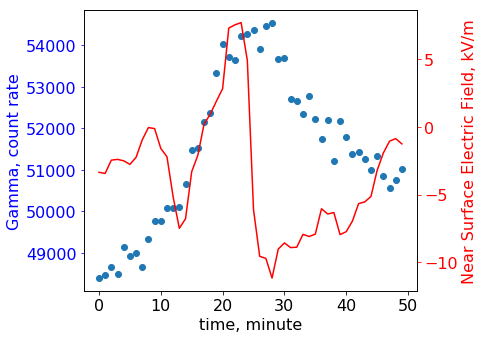
\includegraphics[width=0.5\textwidth]{figures/aragats.png}
	
	
	
	\caption{}
	\label{pic-aragats-a}   
\end{figure}        
\section{Reactor like TGE model}

\section{Proof of concept}
For fast checking the potential of our idea, we considered a next simplified model:  
\begin{itemize}
	\item There are only one tuning parameter  --- the local coefficient of gamma multiplication, describing usefulness of atmosphere for generating secondary particles;
	\item Production of Gamma in cell occurs by Poisson distribution, momentum direction of generated gamma is defined by the electric field direction;
	\item Electric field is chaotic: in point of cell ignition, direction of field is generated by uniform distribution, but magnitudes is constant for whole cloud;
	\item Energy of particle not taken into account, propagation of gamma simulated with exponential distribution with fixed mean free path;
	\item Cloud size is equals 1 kilometer and tracking of particle leaving volume stopped. 
\end{itemize}
    This model is implemented as program on Kotlin programming language.% make url
    
    \section{Results}

    The first figure shows the case of an explosive growth in the number of secondary photons that are well suited to the phenomenon of TGF.
        
    The second figure demonstrates the case when there was a dissipation of an avalanche that had just begun to develop.
       
    The third figure demonstrates the case of a slower and less intensive growth. Such processes with some minor adjustments and assumptions about field dynamics could describe TGE phenomenon.
    
\begin{figure}[ht!]
	\begin{subfigure}[b]{0.5\textwidth}
		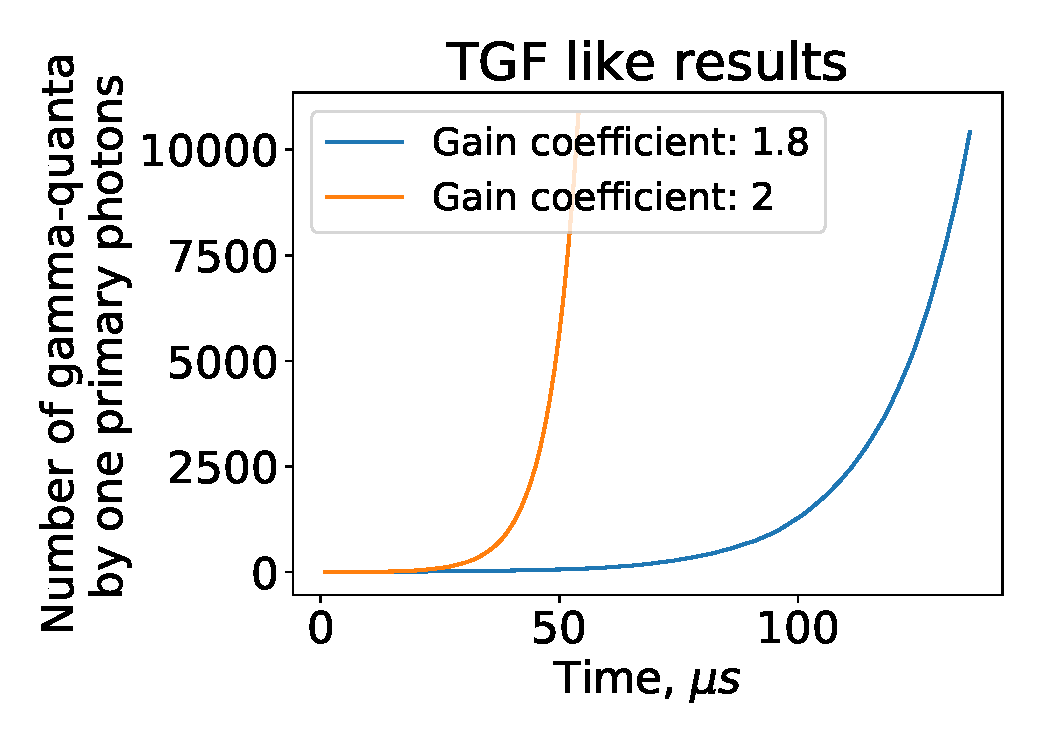
\includegraphics[width=0.95\linewidth]{figures/proofTGF.pdf}
		\caption{}
		\label{pic-tgf-a}
	\end{subfigure}
	~
	\begin{subfigure}[b]{0.5\textwidth}
		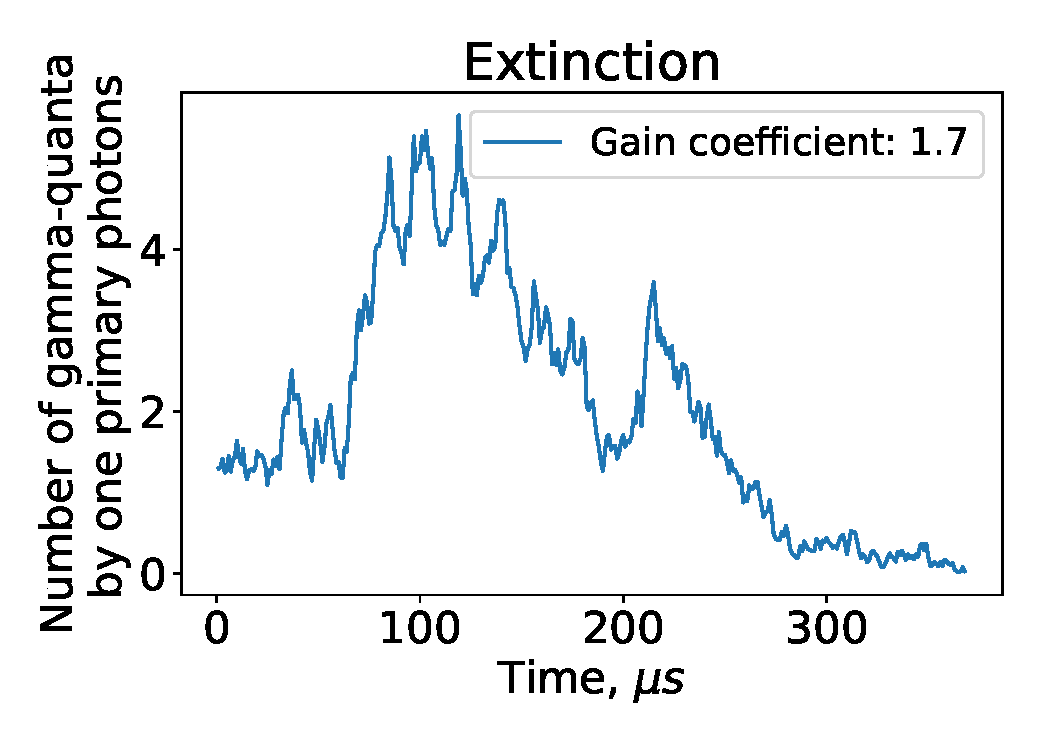
\includegraphics[width=0.95\textwidth]{figures/Extinction.pdf}
		\caption{}
		\label{pic-ext-b}
	\end{subfigure}
	\caption{}
\end{figure}

\begin{figure}[ht!]
	\begin{subfigure}[b]{0.5\textwidth}
		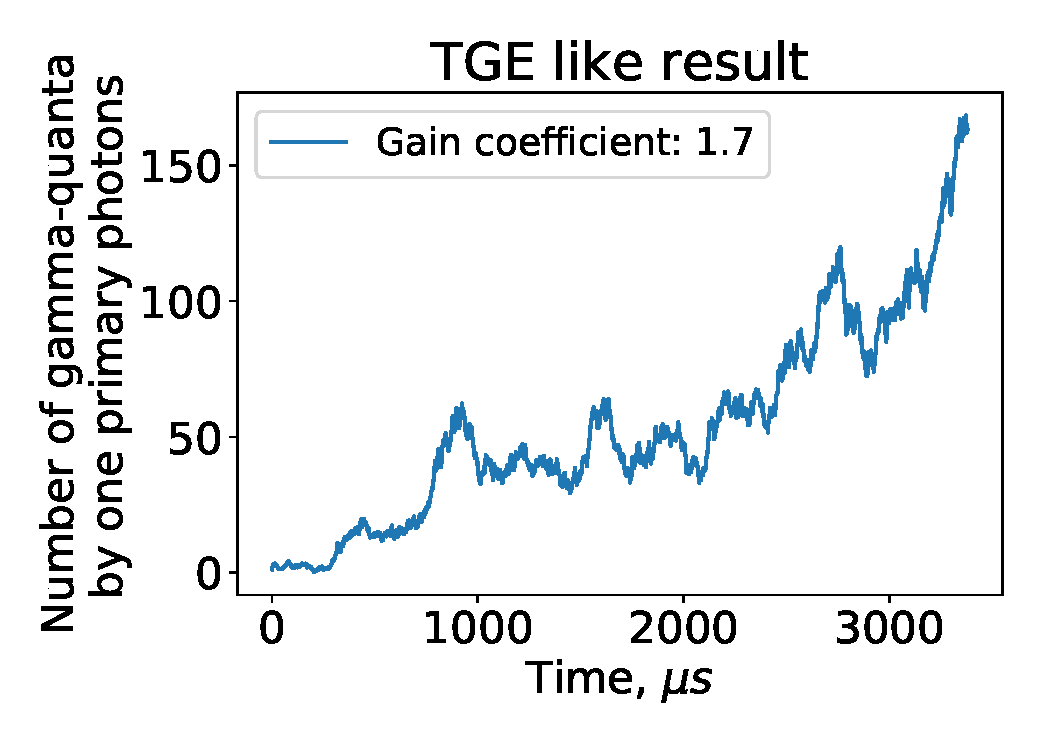
\includegraphics[width=0.95\linewidth]{figures/proofTGE.pdf}
		\caption{}
		\label{pic-tge-a}
	\end{subfigure}
	~
	\begin{subfigure}[b]{0.5\textwidth}
		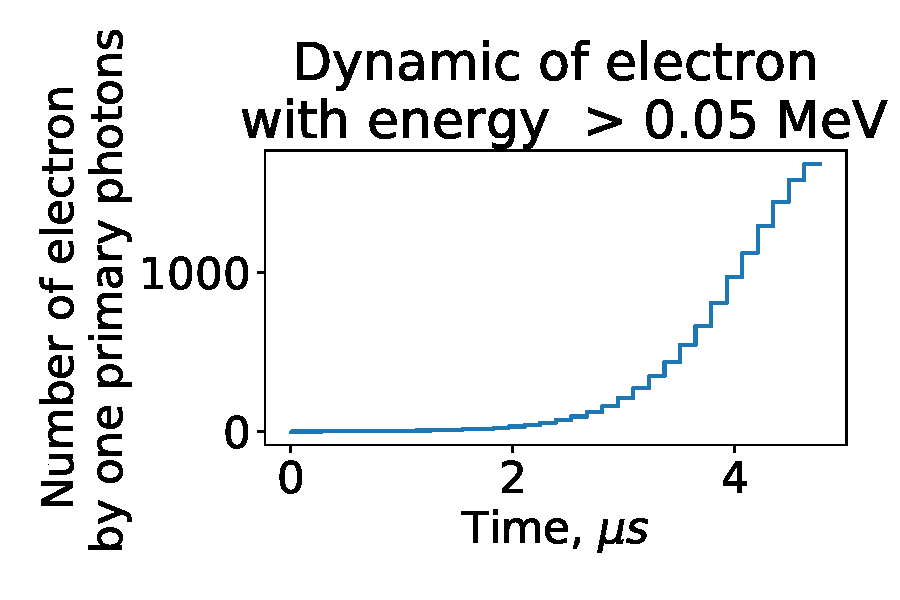
\includegraphics[width=0.95\textwidth]{figures/kotlinElectron.pdf}
		\caption{}
		\label{pic-electron-b}
	\end{subfigure}
	\caption{}
\end{figure}
    \section{Conclusion}
    \begin{itemize}
    	\item Reactor-like model is very good to describe TGF and other fast processes;
    	\item Slow processes like TGE could be described with additional assumptions about field dynamics;
    	\item The model could describe both TGE and TGF with the same mechanism depending on the state of the cloud.
    \end{itemize}
Also reactor like model give next experimentally verifiable consequences:
    \begin{itemize}
    	\item Contrary to Dweyer and unmodified Gurevitch models, reactor model predicts quasi-isotropic (according to field distribution) emmittance of gamma-rays from a thundercloud.  	Measurement of the angular distribution of gamma-rays is required to proove or disproove the concept
    	
    	\item At first approximation, the energy spectrum of photons produced in RL model does not depend on radiation intensity (the spectrum depends on cell field and intensity on cell number).
    \end{itemize}
Moreover reactor like TGE model can be used to investigate intercloud interaction.
\\
This work is supported by the Russian Science Foundation under grant No. 17-12-01439.
    
    \bibliography{references}{}
\end{document}
